% Dokumentenart und Schriftgröße
\documentclass[
    12pt,
    a4paper
]{article}

% Verfügbarmachen externer Funktionalitäten
\usepackage[
    left=4cm,
    right=1.5cm,
    top=3cm,
    bottom=2cm
]{geometry}
\usepackage[
    toc,
    style=alttree,
    acronym,
    nopostdot,
    nonumberlist
]{glossaries}
\usepackage[ngerman]{babel}
\usepackage[export]{adjustbox}
\usepackage[titles]{tocloft}
\usepackage[
    backend=biber,
    style=numeric
]{biblatex}
\usepackage[T1]{fontenc}
\usepackage{verbatim}
\usepackage{minted}
\usepackage{hyperref}
\usepackage{setspace}
\usepackage{graphicx}
\usepackage{ragged2e}
\usepackage{fontspec}
\usepackage{fancyhdr}
\usepackage{svg}
\usepackage{tocbibind}
\usepackage{float}

% Variableneinbindung
% Praxisphasentitel, z. B. 1. Praxisphase im WS 22/23
\newcommand{\phasetitle}{Projektstudium im SS 23}
% Thema der Praxisarbeit
\newcommand{\topic}{Thema der Praxisphase}
% Name des Studenten
\newcommand{\studentname}{Max Mustermann}
% Straße und Hausnummer
\newcommand{\studentstreet}{Musterstraße 1}
% Postleitzahl und Ort
\newcommand{\studentcity}{12345 Musterstadt}
% Matrikelnummer
\newcommand{\studentid}{123456789}
% Hochschulbetreuer
\newcommand{\universitysupervisor}{Prof. Dr. Hans Meier}
% Fachbetreuer
\newcommand{\companysupervisor}{Herr Frank Müller}
% Unternehmen/Behörde
\newcommand{\company}{Hessisches Competence Center für Neue Verwaltungssteuerung, Wiesbaden}
% Datum der Einreichung
\newcommand{\datesubmission}{01.01.2023}

% Einstellungen
% Datei, welche die Einträge für das Literaturverzeichnis enthält
\addbibresource{bibliography.bib}

% Pfad zu Bildern setzen
\graphicspath{{img/}}

% Abkürzungsverzeichnis
\makeglossaries

% Einrückungen im Abbildungsverzeichnis verhindern
\renewcommand\cftfigindent{0pt}

% Seitenzahl in oberer rechter Ecke einblenden
\pagestyle{fancy}
\fancyhf{}
\fancyhead[R]{\thepage}
\renewcommand{\headrulewidth}{0pt}

% Schriftart des Dokuments
\setmainfont{Arial}

% Zeilenabstand
\setstretch{1.5}

% Design des Syntax-Highlightings
\usemintedstyle{staroffice}

% Inhaltsverzeichnis ohne Punkte zwischen Überschrift und Seitenzahl
\renewcommand{\cftdot}{}

% PDF
\hypersetup{
    colorlinks=true,
    citecolor=black,
    linkcolor=black,
    urlcolor=blue,
    pdftitle={Projektstudium im SS 23}
}

% Liste verwendeter Abkürzungen
\newacronym{hcc}{HCC}{Hessisches Competence Center}

\begin{document}

% Seitennummerierung deaktivieren
\pagenumbering{gobble}

% Deckblatt
% Logo-Bereich
\noindent
\begin{minipage}[t]{\textwidth}
    \raisebox{-0.28cm}{\includesvg[height=1.7cm]{logo_thm}}
    \hfill
    \includesvg[height=1.7cm]{logo_sp}
\end{minipage}\\[.5cm]

\begin{Center}
    \textbf{\phasetitle\\[1cm]}
\end{Center}

\noindent
Thema:\\
\textbf{\topic\\[1.5cm]}

% Angaben zum Studenten und der Behörde
\begin{FlushLeft}
    \begin{tabular}{@{} l @{\hspace{2.5cm}} p{.5\linewidth} @{}}
        Vorgelegt von:     & \studentname          \\
                           & \studentstreet        \\
                           & \studentcity          \\
        Matrikelnummer:    & \studentid            \\[1.5cm]
        Eingereicht bei                            \\
        Hochschulbetreuer: & \universitysupervisor \\
        Fachbetreuer:      & \companysupervisor    \\[1.5cm]
        Behörde:           & \company              \\
        Eingereicht am:    & \datesubmission
    \end{tabular}
\end{FlushLeft}

\clearpage

% Seitennummerierung mit großen römischen Zahlen
\pagenumbering{Roman}

% Inhaltsverzeichnis
\tableofcontents

\clearpage

% Angaben zum Abkürzungsverzeichnis
\glsfindwidesttoplevelname
\printglossary[
    type=\acronymtype,
    title=Abkürzungsverzeichnis,
    toctitle=Abkürzungsverzeichnis
]

\clearpage

% Abbildungsverzeichnis
\listoffigures

\clearpage

% Seitennummerierung mit arabischen Zahlen
\pagenumbering{arabic}

\section{Einleitung}
\subsection{Hessisches Competence Center}
Das 2001 gegründete Hessische Competence Center für Neue Verwaltungssteuerung in Wiesbaden (\acrshort{hcc}) ist ein SAP-,
Finanz- und Beschaffungsdienstleister,
der die rund 800 hessischen Landesdienststellen unterstützt \cite{hcc-ueber-uns}.

\begin{figure}[H]
    \centering
    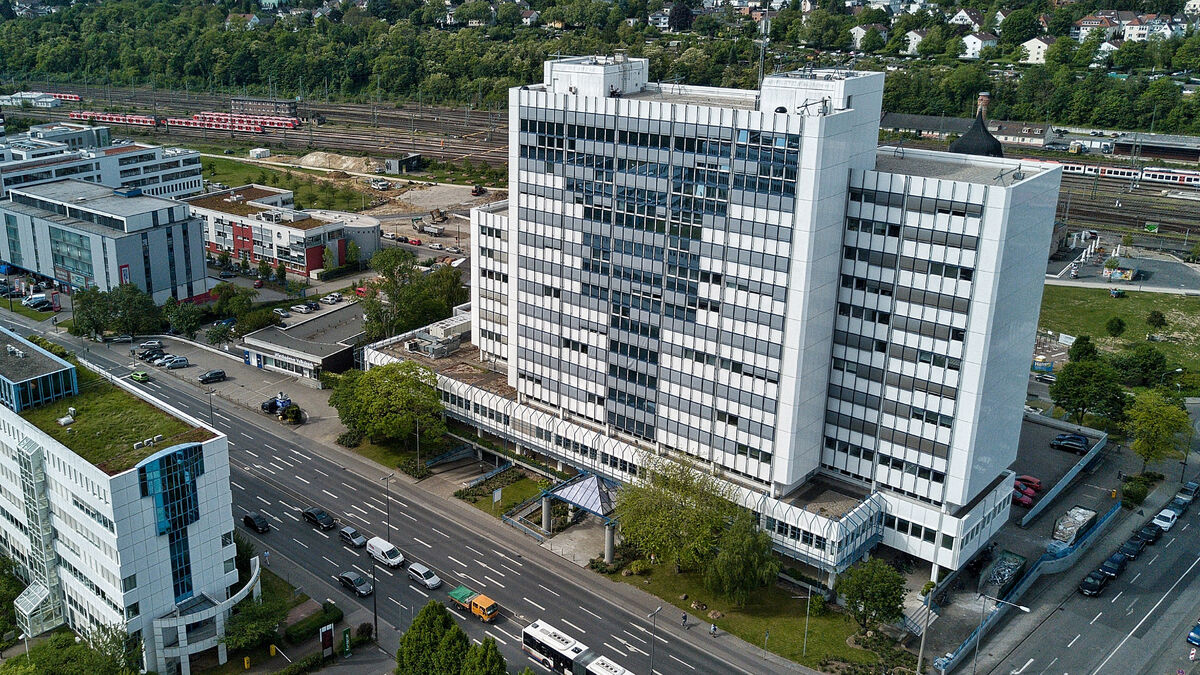
\includegraphics[width=\textwidth]{hcc.jpg}
    \caption{\acrlong{hcc}}
\end{figure}

\clearpage

\pagenumbering{Roman}

% Seitenzahl festlegen
\setcounter{page}{4}

% Literaturverzeichnis
\printbibliography[
    title=Literaturverzeichnis,
    heading=bibintoc
]

\end{document}